\documentclass[11pt]{amsart}

\usepackage{xcolor}
\usepackage{tcolorbox}
\usepackage{geometry}                % See geometry.pdf to learn the layout options. There are lots.
\geometry{letterpaper}                   % ... or a4paper or a5paper or ... 
%\geometry{landscape}                % Activate for for rotated page geometry
%\usepackage[parfill]{parskip}    % Activate to begin paragraphs with an empty line rather than an indent
\usepackage{graphicx}
\usepackage{amssymb}
\usepackage{etoolbox}
\usepackage{pifont}
\newcommand{\cmark}{\ding{51}}%
\newcommand{\xmark}{\ding{55}}%
\usepackage{epstopdf}
\usepackage{tikz}

\usepackage{bibspacing}
\setlength{\bibitemsep}{.82\baselineskip plus .65\baselineskip minus .05\baselineskip}

\DeclareGraphicsRule{.tif}{png}{.png}{`convert #1 `dirname #1`/`basename #1 .tif`.png}

\title{On Bayesian g-Computation and Instrumental Variables for observational data}
\author{P. Gustafson  and H. Campbell}
%\date{}                                           % Activate to display a given date or no date
\setlength{\parskip}{\baselineskip}%
\setlength{\parindent}{0pt}%


\newcommand\independent{\protect\mathpalette{\protect\independenT}{\perp}}
\def\independenT#1#2{\mathrel{\rlap{$#1#2$}\mkern2mu{#1#2}}}

\usepackage{setspace}
\usepackage{etoolbox}
\usepackage{lipsum}

\AtBeginEnvironment{tabular}{\doublespacing}
\begin{document}
\maketitle


\section{Introduction}
\nocite{*}


The power of instrumental variable is discussed in Burgess (2014) \cite{burgess2014sample}.


\begin{table}[h]
\caption{default}
\begin{center}
\begin{tabular}{|c|c|c|}
\hline
& $H=1$& $H=1$  \\
& $A_{0}=0$& $A_{0}=1$  \\
& $P(A_{1}=1)$  & $P(A_{1}=1)$\\
\hline
$L_{1}=0$ & 0.7  & 1\\
$L_{1}=1$ & 0.2  & 1\\
\hline
\end{tabular}
\end{center}
\label{default}
\end{table}%



\begin{table}[h]
\caption{default}
\begin{center}
\begin{tabular}{|c|c|}
\hline
& $P(A_{0}=1)$\\
\hline
$H=0$ & 0.05  \\
$H=1$ & 0.50  \\
\hline
\end{tabular}
\end{center}
\label{default}
\end{table}%

During the study observation period, 23.8\% of patients (Table 1) had been exposed to a DMD, cytotoxic immunosuppressant or other clinical trial drugs. The percentage of treated patients was 1.0\%, 8.3\%, 24.2\%, and 43.4\% for the earliest to the most recent time interval, respectively. However, the actual proportion of the observation time exposed to drug was only 7.0\% overall, and 0.2\%, 1.4\%, 5.0\%, and 16.0\% for the earliest to most recent time-period group, respectively.




Lee \cite{leestructural}  \cite{lee2012finding} considers Instrumental Variable (IV) analysis as an alternative to $g$-computation and discusses how effects can be ``direct'' or ``indirect''.

\begin{figure}[h!]
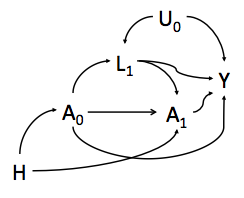
\includegraphics[width=8cm]{figure1.png}
\centering
\end{figure}

http://andrewgelman.com/2015/03/20/bayesian-models-causal-inference-time-varying-exposures/

Given the following change in uptake from period 1 to period 2, what is the required sample size, $n$, to obtain 80\% (90\%) power by instrumental variable analysis.

Similar research for power of IV analysis :

Brion (2013) \cite{brion2013calculating}: Calculating statistical power in Mendelian randomization studies.

Burgess(2014) \cite{burgess2014sample}: ``Sample size and power calculations in Mendelian randomization with a single instrumental variable and a binary outcome'';

Pierce (2010) \cite{pierce2010power}:

``Power and instrument strength requirements for Mendelian randomization studies using multiple genetic variants''

and \cite{pierce2013efficient}.


To verify the IV assumptions :  Glymour (2012) \cite{glymour2012credible}.

For a given effect size, $\delta$, in order to obtain 80\% power, one needs a sample size of approximately XX for successful g-computation.


Examples of calendar period as instrumental variables:  Chen (2011) \cite{chen2011comparative}.


Treatment effect analysis is possibly the most important area in science, because an important reason to do science is to change a cause to improve the outcome. Much of the literature is concerned with ?one-shot? static treatment. But many treatments are repeated over time in reality and, when this is done, they are often modified depending on the interim outcomes. This is natural, as people always try to do better given the information at hand that accumulates over time, and the interim outcomes are part of the information.


Clinical trials are often not practical for long�-term outcomes.  As such, researchers often find themselves in the difficult position of relying on observational data for determining the effect, or lack thereof, of a given exposure,  Shinozaki (2014) \cite{shinozaki2014estimation}.  The primary obstacle for such efficacy studies is that of uncontrollable bias due to confounding by indication (exposure is correlated with an unmeasured predisposition to a given outcome), McMahon (2000) \cite{mcmahon2000design}.  

Even in situations when all possibles confounders are recorded in the data, adjusting for these may not alleviate one of potential bias, if treatment or exposure is time-varying, \cite{robins1999estimation}.  Robbins (1992) identifies two situations in which biased results will occur:

\begin{itemize}
\item{there exists a time-dependent factor that impacts the outcome while also impacting subsequent treatment;}
\item{past treatment history predicts subsequent risk factor level.}
\end{itemize}
The main obstacles with the analysis of time-varying observational data is the presence of: (1) unknown confounders and (2) known time-dependent confounders affected by prior components of the exposure, ``causal intermediates'', Daniel (2013) \cite{daniel2013methods}.    While standard regression models can adequately adjust for confounding of fixed-time variables, adjusting for causal intermediates may not be appropriate, and result in misleading inference, Weinberg(1993) \cite{weinberg1993toward}, Rosenbaum (1984) \cite{rosenbaum1984consquences}.

One strategy is to apply \textbf{$g$-computation}, Borsi (2012) \cite{borsi2012estimating}.  Another, seemingly cruder strategy, would involve treating calendar period of reaching eligibility for treatment as an \textbf{instrumental variable}, Greenland (2000) \cite{greenland2000introduction}.

Note: non-parametric g-computation is identical to IPW:

When all models are nonparametric, the two approaches are identical, as was noted  by Hern�n et al. [8] when first introducing IPW of MSMs.

Robins in his original paper [1] highlighted a problem with the parametric version of the g-computation formula described above, the g-null paradox.



The theoretical properties of the \textbf{$g$-computation} approach have been previously examined, see Johnston et al. (2008) \cite{johnston2008use},  and applications exist across a wide range of disciplines: assessing the the effect of antiretroviral therapy on incident AIDS, Cain et al. (2009) \cite{cain2009effect}; estimating the risk of coronary heart disease, Taubman (2009), \cite{taubman2009intervening}; determining the effect of pillbox organizer use on adherence and viral suppression, Petersen (2007) \cite{petersen2007pillbox}; evaluating time trends in associations between ozone concentrations and hospitalization for asthma, Moore (2008) \cite{moore2008ambient}.   The \emph{Bayesian} $g$-computation, while not as prevalent in the literature, shows promise,  Gustafson (2015) \cite{gustafson2015discussion}, Wang (2011) \cite{wang2011estimating}, Keil (2015) \cite{keil2015bayesian}.  Whether one uses the frequentist or bayesian framework, the validity of the g-computation approach relies on the assumption that all� confounders are measured in the data.

The alternative \textbf{instrumental variable} strategy circumvents the requirement that all confounders are known and measured at the  cost of inducing exposure misclassification, Cain et al. (2009) \cite{cain2009effect}.  Three important assumptions are required:  1. calendar periods are associated with therapy because therapies were introduced sequentially over time; 2. calendar period cannot be affected by indications for treatment with therapy; and 3. calendar period is independent of outcome given indications for and actual use of therapy.  The strength of the instrument (calendar period) is determined by the correlation between exposure and calendar period, with strong instruments being preferable, Johnston and Gustafson (2008) \cite{johnston2008use}.

\textbf{Application-}  Since they were approved 20 years ago, the proportion of MS patients taking beta�-interferons has gone up dramatically, but outcomes, as measured by time from disease onset to  disease progression, have not improved substantially over calendar time.  
Tremlett et el. (2008) \cite{tremlett2008natural} and Tremlett et el. (2010) \cite{tremlett2010new} review recent advances in the understanding of the natural history of MS.
 In order to determine whether or not beta�-interferons are an effective treatment, one can look over extensive subject-level observational data, as in the analysis of Karim et al. (2014) \cite{karim2014marginal}.  If calendar time can be considered an ``instrumental variable'', other methods of analysis may prove advantageous.
  


This paper investigates the merits of each approach in terms of power to detect efficacy (or lack thereof) and robustness to violations of assumptions.



\section{Calendar period as instrumental variable}

\textbf{Cain et al. (2009) \cite{cain2009effect}:}

Simple calendar period approaches may circumvent confounding by indication at the cost of inducing exposure misclassification. To correct this misclassification, the authors propose an instrumental-variable estimator analogous to ones previously used for noncompliance corrections in randomized clinical trials.

These studies used calendar period as a proxy for actual HAART use to circumvent confounding by indication (3). To the extent that calendar period is a misclassified version of actual HAART exposure, estimates using calendar period may be subject to information bias (M. A. Hernan, Harvard School of Public Health, unpublished manuscript, 2009).

3 assumptions of an instrumental variable:

1.  calendar periods are associated with therapy because therapies were introduced sequentially over time. 

2.  calendar period cannot be affected by indications for treatment with therapy.

3.  calendar period is independent of outcome given indications for and actual use of therapy.

calendar period has been used as an instrument in cancer research (\cite{brenner2002long}), and geographic location has been used as an instrument in cardiovascular research (\cite{stukel2007analysis}). 

\textbf{Johnston and Gustafson (2008) \cite{johnston2008use}:}

Given an outcome measure, a treatment variable, a set of unmeasured confounders, and, possibly, a set of measured confounders, a variable satisfies the conditions of an instrumental variable (also referred to as an instrument) if the following conditions hold: 

(1) it is correlated with the treatment variable; 

(2) given the treatment variable and all confounders (measured and unmeasured), it is conditionally independent of outcome; and 

(3) it is independent of the entire set of unmeasured confounders [4]. 

The strength of the instrument is determined by the correlation between treatment and instrument, with strong instruments being preferable.

\textbf{Stukel (2007) \cite{stukel2007analysis}:}

``The instrumental variable behaves like a natural randomization" of patients to regional `treatment groups'
that differ in likelihood of receiving cardiac catheterization. Unlike randomization,
the difference in likelihood of treatment is not 100\%, and one can explore
but not prove that the groups are similar in unmeasured patient characteristics.''


\section{Bayesian g-computation}

\textbf{Vansteelandt and Keiding (2010) \cite{vansteelandt2011invited}:}
Invited Commentary: G-Computation: Lost in Translation?

\textbf{Daniel (2011) \cite{daniel2011gformula}}:

This article describes the gformula command, an implementation of the g-computation procedure, used to estimate the causal effect of time-varying exposure(s) on an outcome in the presence of time-varying confounders that are themselves also affected by the exposure(s). \textbf{The procedure can also be used to address the related problem of estimating controlled direct effects and natural direct/indirect effects when the causal effect of the exposure(s) on an outcome is mediated by intermediate variables, and in particular when confounders of the mediator-outcome relationships are themselves affected by the exposure(s).} A brief overview of the theory and a description of the command and its options are given, and an illustration using two simulated examples is provided.

\textbf{Snowden (2011) \cite{snowden2011implementation}:}

The growing body of work in the epidemiology literature focused on G-computation includes theoretical explanations of the method but very few simulations or examples.  The authors provide a step-by- step demonstration of G-computation that is intended to familiarize the reader with this procedure. 

The distinction between marginal and conditional parameters is important, as it further highlights the limitations of a traditional regression approach when a population-level estimate is of interest.

\textbf{Neugebauer (2007) \cite{neugebauer2007causal}:}

Beyond allowing a more flexible causal analysis, HRMSMs improve computational tractability and mitigate statistical power concerns when designing longitudinal studies. We also develop three consistent estimators of HRMSM parameters under sufficient model assumptions: 

1) the Inverse Probability of Treatment Weighted (IPTW), 

2) G-computation and 

3) Double Robust (DR) estimators.



\textbf{Park and Kaplan (2015) \cite{park2015bayesian}:}

A fully Bayesian approach to causal mediation analysis for group-randomized designs is presented. A unique contribution of this article is the combination of Bayesian inferential methods with G-computation to address the problem of heterogeneous treatment or mediator effects.

The results of the first simulation study demonstrate that our proposed Bayesian approach to causal mediation analysis satisfies Bayesian as well as frequentist properties. The second simulation study suggests that the proposed approach provides unbiased results even under heterogeneous treatment or mediator effects by using G-computation as long as models are correctly specified.

\textbf{Keil (2014) \cite{keil2014parametric}:}

Unlike standard regression approaches, the parametric g-formula can be used to adjust for time-varying confounders that are affected by prior exposures. To date, there are few published examples in which the method has been applied.

Epidemiologists often use regression models (for example, the Cox proportional hazards model) to adjust for confounding; this is equivalent to estimating stratum-specific hazard ratios and then averaging the information-weighted hazard ratios. When some of those confounders are also causal intermediates, this amounts to adjusting away some of the effect of exposure (Weinberg(1993) \cite{weinberg1993toward}, Rosenbaum (1984) \cite{rosenbaum1984consquences}). The g-formula works differently: first, one finds weighted averages of the stratum-specific hazards, and then those averaged (standardized) hazards are combined in a summary hazard ratio. Thus, bias resulting from time-varying covariates that can be both confounders and causal intermediates is a shortcoming of using regression models to control for confounding, rather than a general principle of observational data analysis. The g-formula is a tool that overcomes this shortcoming, but its use in the literature has been sparse -- we could find only 9 examples using observational data.


\textbf{Keil (2015) \cite{keil2015bayesian}:}

Bayesian approaches have shown promise for dealing with under-identified models in environmental epidemiology through the use of parameter prior distributions to stabilize estimates that would be highly variable (or possibly inestimable) in an unpenalized maximum likelihood procedure 


Because standard g-formula algorithms typically require large Monte Carlo samples and a non-parametric bootstrap, the use of MCMC machinery in the Bayesian g-formula does not result in a substantial computational burden relative to the frequentist approach.

As in our time-fixed simulations, under moderately informative, null priors, the bias was larger and the variance was smaller for the Bayesian g-formula than for the standard g-formula. The Bayesian g-formula under moderately informative priors outperformed the standard g-formula at sample sizes under 100 (with respect to MSE), suggesting that the utility of the Bayesian g-formula increases with reasonable, prior information (Table 2).



With respect to unknown confounders, Recently, Bayesian methods have been proposed to address McCandless (2007)\cite{mccandless2007bayesian}.


\section{Applications}


\textbf{Cole (2013) \cite{cole2013analysis} :}


Analysis of Occupational Asbestos Exposure and Lung Cancer Mortality Using the G Formula

The G null paradox states that, under the null hypothesis, it may be impossible to correctly specify the parametric models required for the G formula (11). There- fore, in large samples, the parametric G formula may reject the null hypothesis, even when it is true. In our context we are not overly concerned about the G null paradox, because asbestos is an established cause of lung cancer (31).

Future implementations might explore the introduction of prior knowledge into the parametric G formula through Bayesian methods.


\textbf{Taubman (2009) \cite{taubman2009intervening}:}

Unlike standard methods, the parametric g-formula can deliver consistent estimates of risk even when time-dependent confounders are affected by prior components of the intervention; although, in this setting, the parametric g-formula is subject to the `g-null paradox' theorem, which implies it can be essentially impossible to correctly specify the needed parametric models under the causal null hypothesis. As a consequence, the method will reject the causal null, even when true, in sufficiently large samples.

Estimating the population risk of disease under hypothetical interventions -- such as the population risk of coronary heart disease (CHD) were everyone to quit smoking and start exercising or to start exercising if diagnosed with diabetes?may not be possible using standard analytic techniques. The parametric g-formula, which appropriately adjusts for time-varying confounders affected by prior exposures, is especially well suited to estimating effects when the intervention involves multiple factors (joint interventions) or when the intervention involves decisions that depend on the value of evolving time-dependent factors (dynamic interventions). We describe the parametric g-formula, and use it to estimate the effect of various hypothetical lifestyle interventions on the risk of CHD using data from the Nurses' Health Study.

We discuss whether the assumptions required for the validity of the parametric g-formula hold in the Nurses' Health Study data. This work represents the first large-scale application of the parametric g-formula in an epidemiologic cohort study.

\textbf{Petersen (2007) \cite{petersen2007pillbox}:}

Marginal structural models were used to estimate the effect of pillbox organizer use on adherence and viral suppression, adjusting for confounding by CD4+ T cell count, viral load, prior adherence, recreational drug use, demographic characteristics, and current and past treatment.

Three distinct estimators:

1- inverse probability of treatment weighted (IPTW), 

2-G-computation 

3- double robust

G-computation (in the current application) relies on standard multivariable regression of adherence on pillbox organizer use and confounders. IPTW estimation, in contrast, relies on multivariable logistic regression of pillbox organizer use on confounders (the treatment mechanism). 

The double robust estimator makes use of (1) the multivariable regression of adherence on pillbox organizer use and confounders used in G-computation and (2) the multi- variable logistic regression of pillbox organizer use on confounders (treatment mechanism) used in IPTW estimation.

\textbf{Time-lagged confounder measurements were used to ensure that confounders occurred before (and, therefore, could not be influenced by) pillbox organizer use. }


\textbf{Moore (2008) \cite{moore2008ambient}:}

This traditional approach does not answer directly our original question of interest: 

We implemented two estimators of history-restricted marginal structural models (HRMSMs) (Neugebauer et al. 2007) causal parameters: the inverse probability of treatment weighted (IPTW) and G-computation. Confidence intervals (CIs) and p-values for the two estimates were obtained with 10,000 bootstrap iterations, where resampling was based on the 195 independent grids.

We applied a diagnostic tool to assess the bias in the IPTW estimator due to the experimental treatment assignment (ETA) violation (Wang et al. 2006) and showed a 76\% bias in comparison to the G-computation estimate (Table 4). Therefore, we relied on the G-computation estimator.

This would represent the same effect estimated by the conventional regression analysis. In other words, the results from the MSM and conventional analyses, in this particular analysis, give identical parameter estimates because there are no interaction terms in the conventional model.


The results of this analysis indicated that the conventional statistical association model, in this particular analysis, was equivalent to the G-computation estimates of the HRMSM parameters?an observation that is not surprising, given that there were no interactions in the association model. 

\section{df}
    
$\quad$

\begin{table}[h]
\begin{center}
 \begin{tabular}{||c | c c c||} 
 \hline
 & \textbf{IV} & \textbf{$g$-comp with H} & \textbf{$g$-comp without H} \\ [0.5ex] 
  \hline
 \textbf{Assumption} &   & &   \\ 
 \hline\hline
 $H \independent Z$, $\theta_{10} = 0$ &  \checkmark &  \xmark & \checkmark \\
   \hline
  $(H | X, C, Z) \independent Y$, $\theta_{8}=0$& \checkmark & \xmark &  \checkmark  \\ 
 \hline
  H is correlated with X, $\theta_{2} > 0$& \checkmark & \xmark & \xmark  \\ 
 \hline
No unknown confounders, $\theta_{9}=0$& \xmark & \checkmark & \checkmark \\ [0.5ex] 
 \hline\hline
  \textbf{Required Data} &   &  & \\ 
 \hline
 H  & \checkmark & \checkmark &\xmark  \\ 
 \hline
X  & \xmark & \checkmark  & \checkmark \\ 
 \hline
C & \xmark & \checkmark & \checkmark \\
 \hline
\end{tabular}
\end{center}
\caption{Assumptions and required data for both approaches.}
\end{table}



$\quad$

The objective is to determine the significance (superiority or non-inferiority) of the target value $T_{(1,1)-(0,0)}$:

\begin{equation}
T_{(1,1)-(0,0)} =  Pr(Y_{2}=1 | do(X_{1}=1, X_{2}=1))  -   Pr(Y_{2}=1 | do(X_{1}=0, X_{2}=0))
\end{equation}



\newpage


%\begin{figure}[h!]
%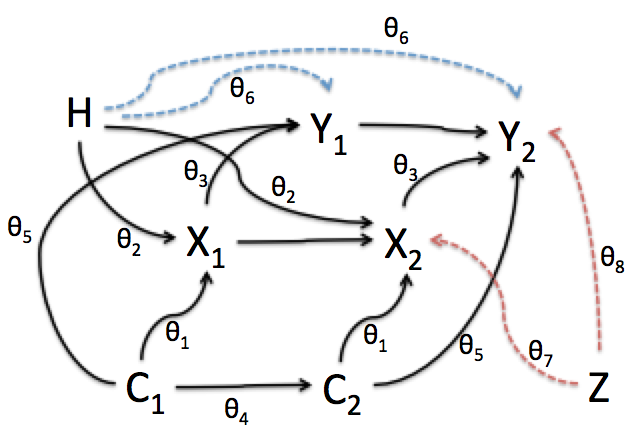
\includegraphics[width=12cm]{mypic2.png}
%\caption{The two time-point model considered.  We do not suggest that this model will be adequate for all applications. However, it is sufficiently rich to provide a vehicle for investigating the consequences of preferential sampling, and for the application that is described in Section X of the paper.}
%\centering
%\end{figure}

\begin{figure}[h!]
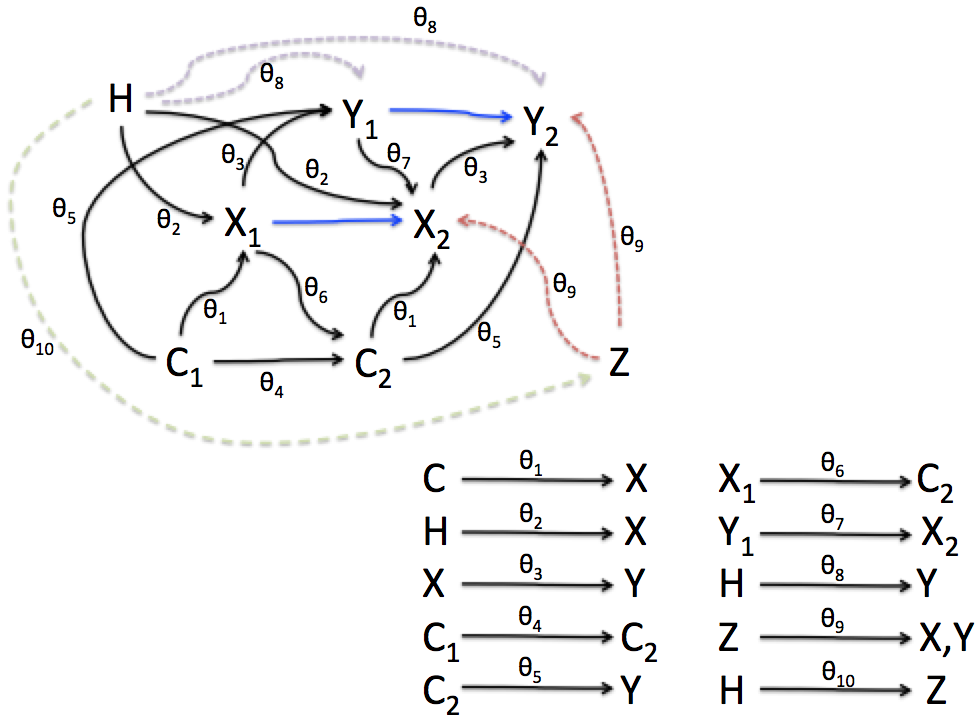
\includegraphics[width=18cm]{modelplot1.png}
\caption{Consider the variables as unfolding in the temporal order (H, C1, X1,Y1,C2,X2,Y2).}
\centering
\end{figure}


$\quad$
\begin{spacing}{1.9}
\begin{table}[h]
\begin{center}
 \begin{tabular}{||c | c c c c||} 
 \hline
  & & & \textbf{Representation} & \textbf{Interpretation} \\ [0.5ex] 
  \hline
 \textbf{Variable} & \textbf{if = 0} & \textbf{if $=$ 1}  &   & \\ 
 \hline\hline
 H & early & late &  Instrumental Variable & Calendar time  \\ 
 \hline
 C & low & high & Known Confounder  & Relapse Rate\\ 
 \hline
 Y & ill & healthy & Outcome of interest  & Disease progression\\ 
 \hline
 Z &  &   & Unknown additional confounder &  \\ 
 \hline
X & no treatment  & treatment & Intervention of interest & Treatment \\ [0.5ex] 
 \hline\hline
 \hline

\end{tabular}
\end{center}
\caption{Model Components.}
\end{table}
\end{spacing}





$\quad$


$\quad$

$\quad$

\newpage

Given an outcome measure, a treatment variable, a set of unmeasured confounders, and, possibly, a set of measured confounders, a variable satisfies the conditions of an instrumental variable (also referred to as an instrument) if the following conditions hold: 

\begin{itemize}
\item{(1) it is correlated with the treatment
variable}
\item{(2) given the treatment variable and all confounders (measured and unmeasured), it is conditionally independent of outcome; and}
\item{(3) it is independent of the entire set of unmeasured
confounders \cite{greenland2000introduction}.}
\end{itemize}

\newpage




 \section{Methods}
 
 
 
 
 \textbf{Frequentist g-comp with logistic model:}
 
 
\begin{tcolorbox}

\begin{enumerate}
\item{  Fit a regression model: $Y_{2} \sim H$}
\item{ Significant association ($Y_{2} \sim H$) $\Rightarrow$ Significant association ($Y_{2} \sim X$)}
\end{enumerate}


\end{tcolorbox}



$\quad$

\textbf{Bayesian g-comp with Uniform priors:}
$Pr(A=1 | B=b, C=c) \sim Beta(1+ \sum_{i=1}^{n}1_{(A=1,B=b,C=c)}(x_{i}), 1+ \sum_{i=1}^{n}1_{(A=0,B=b,C=c)(x_{i})})$

$f(x) = \frac{\Gamma(a+b)}{(\Gamma(a)\Gamma(b))}x^{(a-1)}(1-x)^{(b-1)}$

\begin{tcolorbox}

\begin{enumerate}
\item{ Obtain a sample from the posterior distribution $\gamma$.}
\item{ By summation (integration), use samples of $\gamma$ to obtain samples from the posterior distribution of $ Pr(Y_{2}=1 | do(X_{1}=x_{1}, X_{2}=x_{2}))$}
\item{Calculate posterior predictive $p$-value.}
\end{enumerate}


\end{tcolorbox}


$\quad$



\section{4 $g$-computation models}

\textbf{With $Y_1$, without $H$:}

\begin{align*}
  Pr(Y_{2}=1 | do(X_{1}=x_{1}, X_{2}=x_{2})) & =  \sum_{y_{1}=0}^{1} \sum_{c_{1}=0}^{1} \sum_{c_{2}=0}^{1}
 Pr(C_{1}=c_{1}) \\
 &\cdot   Pr(C_{2}=c_{2} | C_{1}=c_{1}, X_{1}=x_{1}) \\
 & \cdot   Pr(Y_{1}=y_{1} | C_{1}=c_{1}, X_{1}=x_{1}) \\
 &\cdot   Pr(Y_{2}=1 | C_{2}=c_{2}, X_{2}=x_{2}, Y_{1}=y_{1})
\end{align*}

\textbf{With $Y_1$, and with $H$:}

\begin{align*}
  Pr(Y_{2}=1 | do(X_{1}=x_{1}, X_{2}=x_{2})) & =  \sum_{y_{1}=0}^{1} \sum_{c_{1}=0}^{1} \sum_{c_{2}=0}^{1} \sum_{h=0}^{1}
 Pr(H=h) \cdot Pr(C_{1}=c_{1} | H=h) \\
 &\cdot   Pr(C_{2}=c_{2} | C_{1}=c_{1}, X_{1}=x_{1}, H=h) \\
 & \cdot   Pr(Y_{1}=y_{1} | C_{1}=c_{1}, X_{1}=x_{1}, H=h) \\
 &\cdot   Pr(Y_{2}=1 | C_{2}=c_{2}, X_{2}=x_{2}, Y_{1}=y_{1}, H=h)
\end{align*}

\textbf{Without $Y_1$, without $H$:}

\begin{align*}
  Pr(Y_{2}=1 | do(X_{1}=x_{1}, X_{2}=x_{2})) & =  \sum_{c_{1}=0}^{1} \sum_{c_{2}=0}^{1}
 Pr(C_{1}=c_{1}) \\
 &\cdot   Pr(C_{2}=c_{2} | C_{1}=c_{1}, X_{1}=x_{1}) \\
 &\cdot   Pr(Y_{2}=1 | C_{2}=c_{2},C_{1}=c_{1}, X_{2}=x_{2}, X_{1}=x_{1})
\end{align*}

\textbf{Without $Y_1$, with $H$:}

\begin{align*}
  Pr(Y_{2}=1 | do(X_{1}=x_{1}, X_{2}=x_{2})) & =  \sum_{c_{1}=0}^{1} \sum_{c_{2}=0}^{1} \sum_{h=0}^{1}
 Pr(H=h) \cdot Pr(C_{1}=c_{1} | H=h) \\
 &\cdot   Pr(C_{2}=c_{2} | C_{1}=c_{1}, X_{1}=x_{1}, H=h) \\
 &\cdot   Pr(Y_{2}=1 | C_{2}=c_{2}, X_{2}=x_{2}, C_{1}=c_{1}, X_{1}=x_{1}, H=h)
\end{align*}

 
- run down of the simple sandbox of two time-points, everything binary 
	- g-computation (perhaps motivated several different ways)
	- IV idea

Comparison in a focussed scenario
-	confounding by indication present (C encourages treatment start)
-	different possible forms of treatment effect (through C and/or around C)
-	both sets of assumptions met

Comparison across a broad range of scenarios

-	set up distribution giving rise to a wide array of states of the world
-	look for patterns, e.g., is the power of the g-computation driven only by theta11-theta00, or are there other important factors
    
Violations of assumptions

-	any defensible sense of one procedure being more robust than the other
-	how quickly is power lost as we relax assumptions


\begin{figure}[h!]
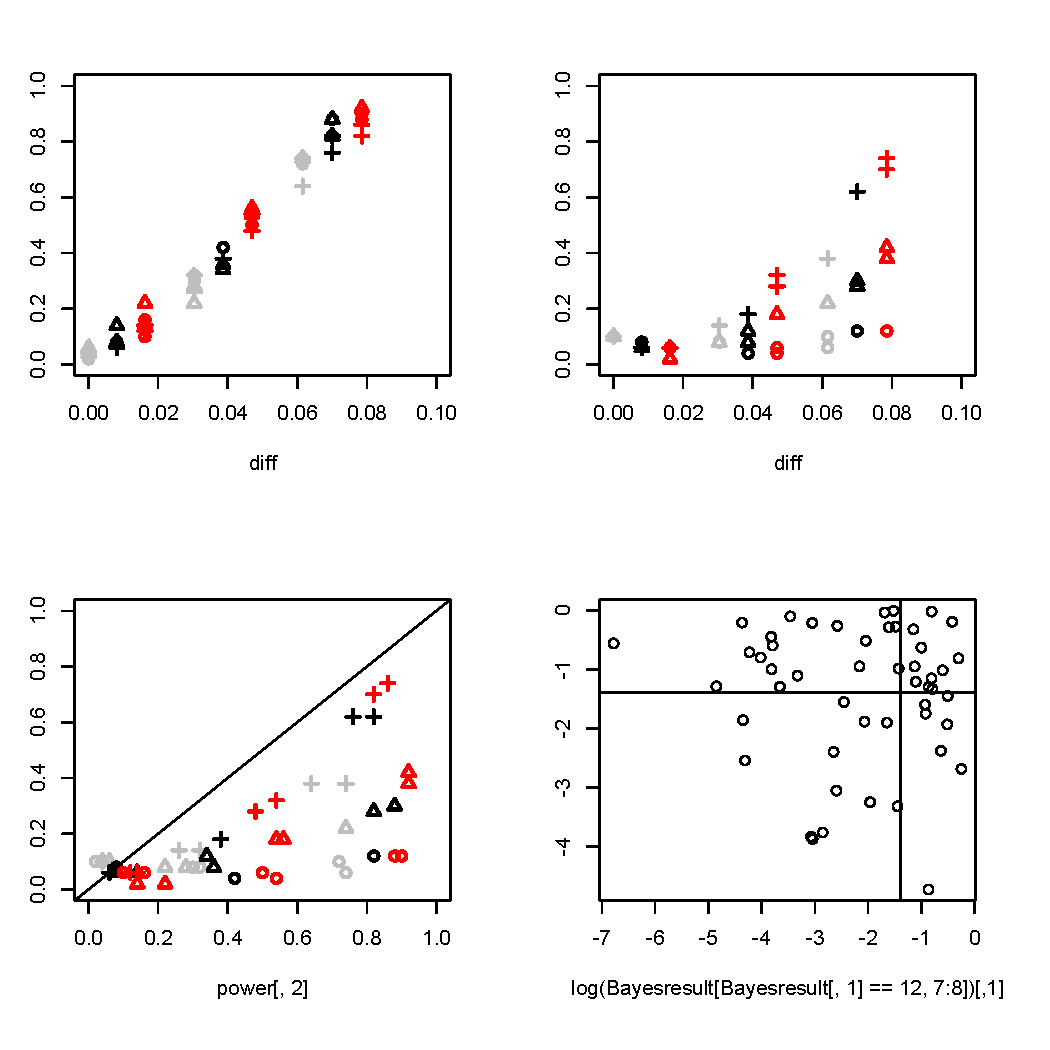
\includegraphics[width=12cm]{RplotPaul.pdf}
\caption{Results of Simulation study.}
\centering
\end{figure}



 \section{Application}

 \section{Discussion}
\newpage

\bibliography{gcomp_refs} 
\bibliographystyle{acm.bst}


\end{document}  